\section{From Basic Waveforms to Musical Perception}
\label{sec:perception}

The previous section described how early sound chips generated a limited set of waveforms under hardware constraints.
These signals become meaningful in music once listeners perceive them; the link between synthesis and musical expression can be summarized by three attributes---timbre, pitch, and loudness.

\subsection{Timbre: Waveform as Sound Color}

Timbre mainly depends on waveform shape.
Even when pitch and loudness match, different waveforms still sound different.
The three primitives on typical 1980s sound chips mapped to distinct musical roles:

\begin{itemize}
  \item \textbf{Square wave.} Produces a clear, distinct tone, suitable for lead melodies and simple harmonies.
  \item \textbf{Sawtooth wave.} Sounds fuller and more stable---often used for bass lines.
  \item \textbf{Noise wave.} Lacks stable pitch---used for percussion and drum-like effects.
\end{itemize}

Figure~\ref{fig:three-waves} illustrates these waveform shapes and their timbral basis.

\subsection{Pitch: Frequency Determines Musical Notes}

Pitch is determined by frequency: a higher carrier frequency is heard as a higher note.
In twelve-tone equal temperament, one semitone corresponds to the frequency ratio $2^{1/12}$, so an interval of $n$ semitones scales frequency by $(2^{1/12})^n$.
Table~\ref{tab:c-major-scale} lists selected C-major scale frequencies as an example.

\begin{table}[htbp]
  \centering
  \caption{Frequencies of selected notes in the C major scale.}
  \label{tab:c-major-scale}
  \begin{tabular}{cccc}
    \toprule
    \textbf{Syllable} & \textbf{Frequency (Hz)} & \textbf{Interval vs.\ prev.} & \textbf{Frequency ratio} \\
    \midrule
    do & 261.63 & --- & --- \\
    re & 293.66 & 2 semitones & $(2^{1/12})^2$ \\
    mi & 329.63 & 2 semitones & $(2^{1/12})^2$ \\
    fa & 349.23 & 1 semitone & $2^{1/12}$ \\
    sol & 392.00 & 2 semitones & $(2^{1/12})^2$ \\
    \bottomrule
  \end{tabular}
\end{table}

As Table~\ref{tab:c-major-scale} shows, note spacing is multiplicative rather than additive in frequency.

\subsection{Loudness: Amplitude Controls Perceived Volume}

Loudness is dominated by amplitude: larger waveform excursions are heard as louder sounds.
Figure~\ref{fig:three-amplitudes} shows three sawtooth waves sharing the same frequency but different peak amplitudes; Table~\ref{tab:loudness-comparison} lists the corresponding amplitude ratios.

The level difference between amplitudes $A_1$ and $A_2$ may be expressed in decibels (dB) as
\[
L = 20 \log_{10}\!\left(\frac{A_2}{A_1}\right).
\]
For amplitude ratios $1{:}2{:}4$, each doubling yields about $6.02~\mathrm{dB}$, as plotted in Figure~\ref{fig:three-amplitudes} and summarized in Table~\ref{tab:loudness-comparison}.
Thus loudness aligns more naturally with a logarithmic amplitude scale than a linear one.

\begin{figure}[htbp]
  \centering
  \subfigure[Amplitude $=0.20$.\label{fig:loudness-1x}]{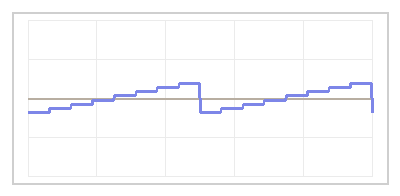
\includegraphics[width=0.32\linewidth]{pictures/loudness_comparison_1x.png}}
  \hfill
  \subfigure[Amplitude $=0.40$.\label{fig:loudness-2x}]{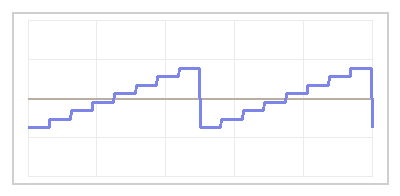
\includegraphics[width=0.32\linewidth]{pictures/loudness_comparison_2x.png}}
  \hfill
  \subfigure[Amplitude $=0.80$.\label{fig:loudness-4x}]{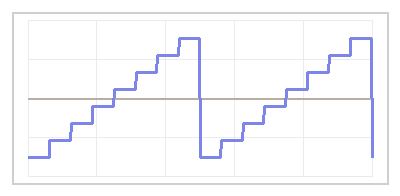
\includegraphics[width=0.32\linewidth]{pictures/loudness_comparison_4x.png}}
  \caption{Sawtooth waveforms at the same frequency with different peak amplitudes.}
  \label{fig:three-amplitudes}
\end{figure}

\begin{table}[htbp]
  \centering
  \caption{Relative amplitude and decibel levels for sawtooth waves with peaks $0.20$, $0.40$, and $0.80$.}
  \label{tab:loudness-comparison}
  \begin{tabular}{cccc}
    \toprule
    Amplitude & Ratio to $0.20$ & Level vs.\ $0.20$ & Increment (dB) \\
    \midrule
    $0.20$ & $1{:}1$ & $0.00$ & --- \\
    $0.40$ & $2{:}1$ & $6.02$ & $6.02$ \\
    $0.80$ & $4{:}1$ & $12.04$ & $6.02$ \\
    \bottomrule
  \end{tabular}
\end{table}
